\documentclass[11pt,a4paper]{article}
\usepackage[utf8]{inputenc}
\usepackage[T1]{fontenc}
\usepackage[margin=2cm]{geometry}
\usepackage{graphicx}
\usepackage{booktabs}
\usepackage[table]{xcolor}
\usepackage{amsmath}
\usepackage{hyperref}
\usepackage{float}
\usepackage{caption}
\usepackage{fancyhdr}
\usepackage{titlesec}
\usepackage{enumitem}
\usepackage{listings}
\usepackage[protrusion=true,expansion=false]{microtype}
\setlength{\headheight}{14pt}

\definecolor{myblue}{RGB}{31,78,121}
\definecolor{codegray}{RGB}{245,245,245}

\hypersetup{
    colorlinks=true,
    linkcolor=myblue,
    urlcolor=myblue
}

\lstset{
    backgroundcolor=\color{codegray},
    basicstyle=\ttfamily\footnotesize,
    breaklines=true,
    frame=single,
    rulecolor=\color{gray!40},
    xleftmargin=5pt,
    xrightmargin=5pt,
    aboveskip=6pt,
    belowskip=6pt
}

\pagestyle{fancy}
\fancyhf{}
\rhead{\textit{Adversarially Robust IDS}}
\lhead{\textit{Deep Learning --- Projet 1}}
\cfoot{\thepage}

\titleformat{\section}{\large\bfseries\color{myblue}}{}{0em}{\thesection\quad}
\titleformat{\subsection}{\normalsize\bfseries\color{myblue!80}}{}{0em}{\thesubsection\quad}

\title{
    \vspace{-1cm}
    {\large Deep Learning en Cybers\'ecurit\'e --- Projet 1}\\[0.4em]
    {\LARGE\bfseries\color{myblue} Adversarially Robust\\Intrusion Detection System}\\[0.6em]
    {\normalsize Dataset : UNSW-NB15 \quad|\quad Attaques : FGSM, PGD \quad|\quad D\'efenses : Adv. Training, Feature Squeezing}
}
\author{Zakariya El Mansouri \quad \texttt{zakariyaelmansouri40@gmail.com}}
\date{Avril 2026}

\begin{document}

\maketitle
\thispagestyle{fancy}

\begin{abstract}
\noindent
Ce rapport pr\'esente la conception d'un syst\`eme de d\'etection d'intrusion (IDS) bas\'e sur un r\'eseau de neurones,
son \'evaluation sous attaques adversariales, et l'efficacit\'e de deux m\'ethodes de d\'efense.
Nous entra\^inons un MLP binaire sur le dataset \textbf{UNSW-NB15} (82\,332 exemples d'entra\^inement,
175\,341 de test, 42 features), puis nous appliquons les attaques FGSM et PGD en respectant un
\emph{threat model} r\'ealiste (seules les features manipulables par l'attaquant sont perturb\'ees).
Deux d\'efenses sont compar\'ees : l'adversarial training et le feature squeezing.
Le feature squeezing obtient le meilleur compromis robustesse/performance,
maintenant un F1 de \textbf{0.852} sous PGD contre \textbf{0.774} pour l'adversarial training.
\end{abstract}

\tableofcontents
\vspace{0.5em}

%% ============================================================
\section{Introduction et Threat Model}
%% ============================================================

Les syst\`emes de d\'etection d'intrusion bas\'es sur l'apprentissage automatique sont vuln\'erables aux
\emph{exemples adversariaux} : des entr\'ees soigneusement perturb\'ees pour tromper le mod\`ele.
Dans un contexte r\'eseau, cela signifie qu'un attaquant peut modifier l\'eg\`erement les statistiques
de son trafic (timing, volume de paquets) pour \'eviter la d\'etection tout en maintenant l'efficacit\'e
de son attaque.

\subsection*{Threat Model}

Nous d\'efinissons pr\'ecis\'ement ce que l'attaquant peut et ne peut pas modifier :

\begin{itemize}[leftmargin=1.5em]
    \item \textbf{Features manipulables} (l'attaquant contr\^ole le timing et le volume) :\\
    \texttt{dur, spkts, dpkts, sbytes, dbytes, sttl, sload, dload, sinpkt, dinpkt, sjit, djit, smean, dmean}
    \item \textbf{Features non manipulables} (changer ces valeurs briserait l'attaque) :\\
    \texttt{proto, service, state, srcip, dstip, dport}
\end{itemize}

L'attaquant op\`ere en \emph{white-box} : il a acc\`es au mod\`ele et peut calculer les gradients.
Son objectif est de faire passer des attaques pour du trafic normal (\emph{evasion attack}).

%% ============================================================
\section{Dataset et Pr\'etraitement}
%% ============================================================

\subsection{Dataset UNSW-NB15}

Le dataset UNSW-NB15 a \'et\'e cr\'e\'e au laboratoire Cyber Range de l'Australian Defence Force Academy.
Il contient du trafic r\'eseau r\'eel captur\'e avec un g\'en\'erateur d'attaques,
couvrant 9 types d'attaques (Fuzzers, Analysis, Backdoors, DoS, Exploits, Generic, Reconnaissance, Shellcode, Worms).

\begin{table}[H]
\centering
\caption{Statistiques du dataset UNSW-NB15}
\begin{tabular}{lrrr}
\toprule
\textbf{Ensemble} & \textbf{Exemples} & \textbf{Attaques (label=1)} & \textbf{Normal (label=0)} \\
\midrule
Train & 82\,332  & 45\,332 (55.1\%) & 37\,000 (44.9\%) \\
Test  & 175\,341 & --- & --- \\
\midrule
\multicolumn{2}{l}{\textbf{Features}} & \multicolumn{2}{r}{42 (num\'eriques + cat\'egorielles)} \\
\bottomrule
\end{tabular}
\end{table}

Les classes sont bien \'equilibr\'ees (55/45), ce qui \'evite les probl\`emes de d\'es\'equilibre classiques.
Parmi les 42 features, certaines discriminent fortement normal vs attaque :
\texttt{ct\_state\_ttl}, \texttt{sttl}, \texttt{dttl}.

\begin{figure}[H]
\centering
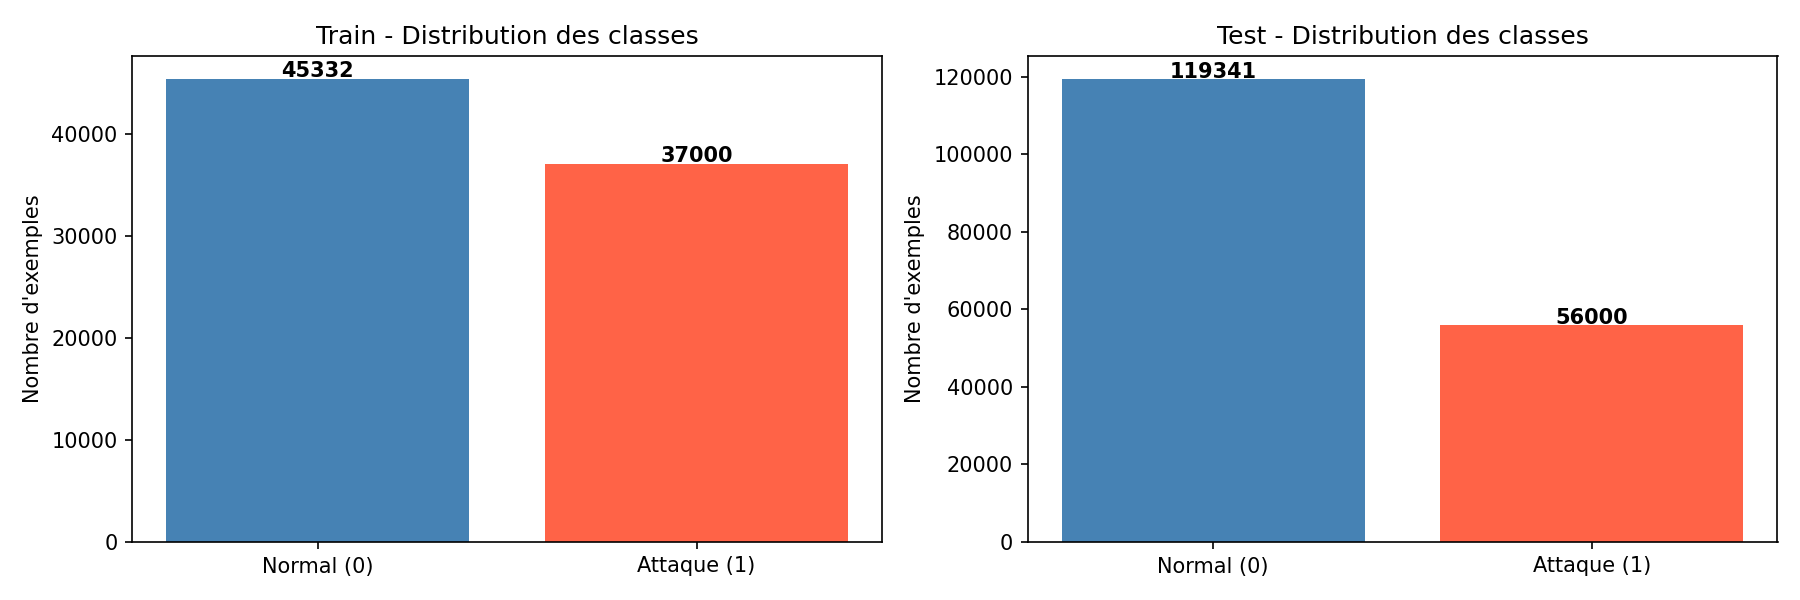
\includegraphics[width=0.48\textwidth]{../results/class_distribution.png}
\hfill
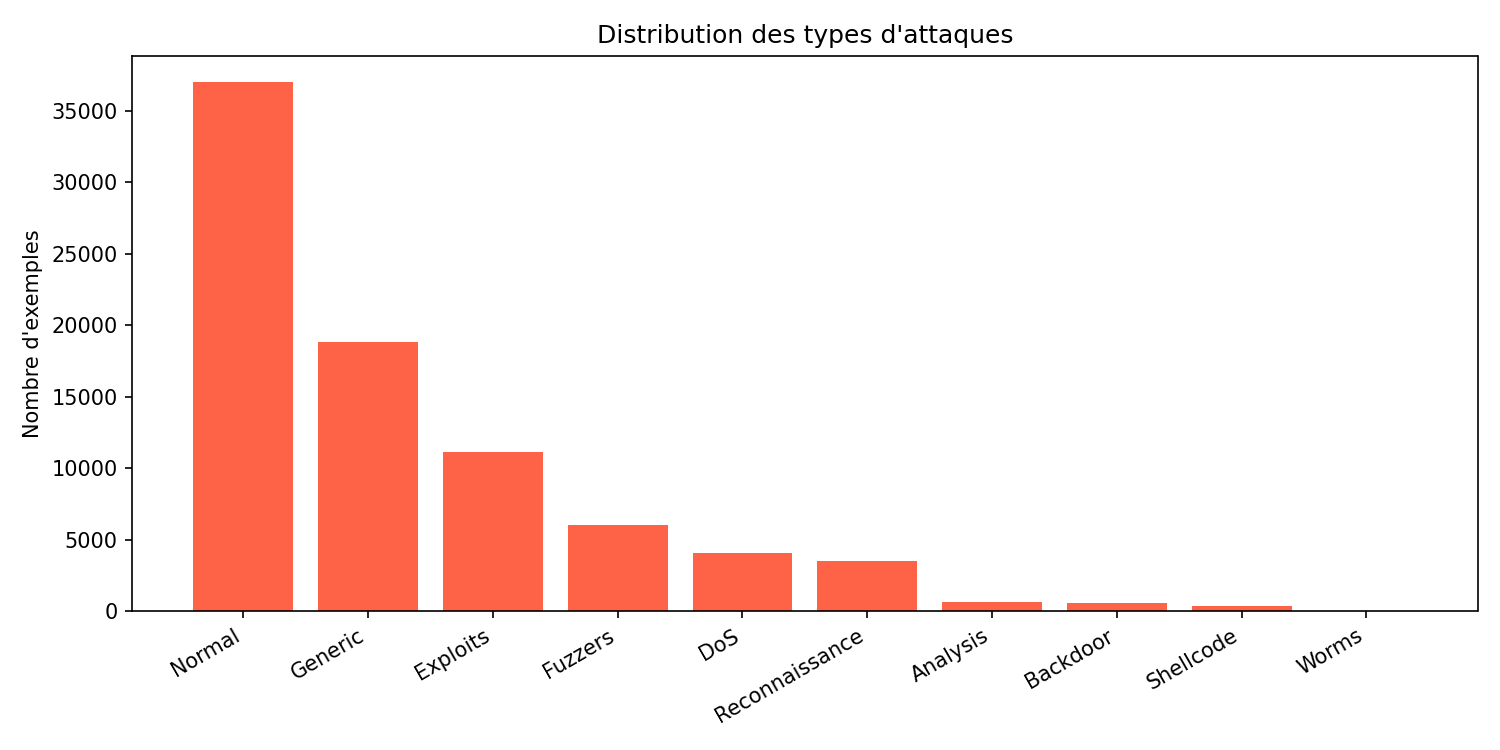
\includegraphics[width=0.48\textwidth]{../results/attack_types.png}
\caption{Distribution des classes (gauche) et types d'attaques (droite)}
\end{figure}

\subsection{Pipeline de pr\'etraitement}

\begin{enumerate}[leftmargin=1.5em]
    \item \textbf{Suppression des colonnes inutiles} : \texttt{id}, \texttt{attack\_cat}
    \item \textbf{Gestion des valeurs manquantes/infinies} : remplacement par la m\'ediane du train
    \item \textbf{Encodage des variables cat\'egorielles} : \texttt{LabelEncoder} sur \texttt{proto}, \texttt{service}, \texttt{state}
    \item \textbf{Normalisation} : \texttt{StandardScaler} (moyenne = 0, \'ecart-type = 1) ajust\'e sur le train uniquement
\end{enumerate}

La normalisation est indispensable : sans elle, une feature avec des valeurs $[0, 10^5]$
dominerait une feature $[0, 1]$ et le mod\`ele apprendrait des corr\'elations artificielles.

\begin{figure}[H]
\centering
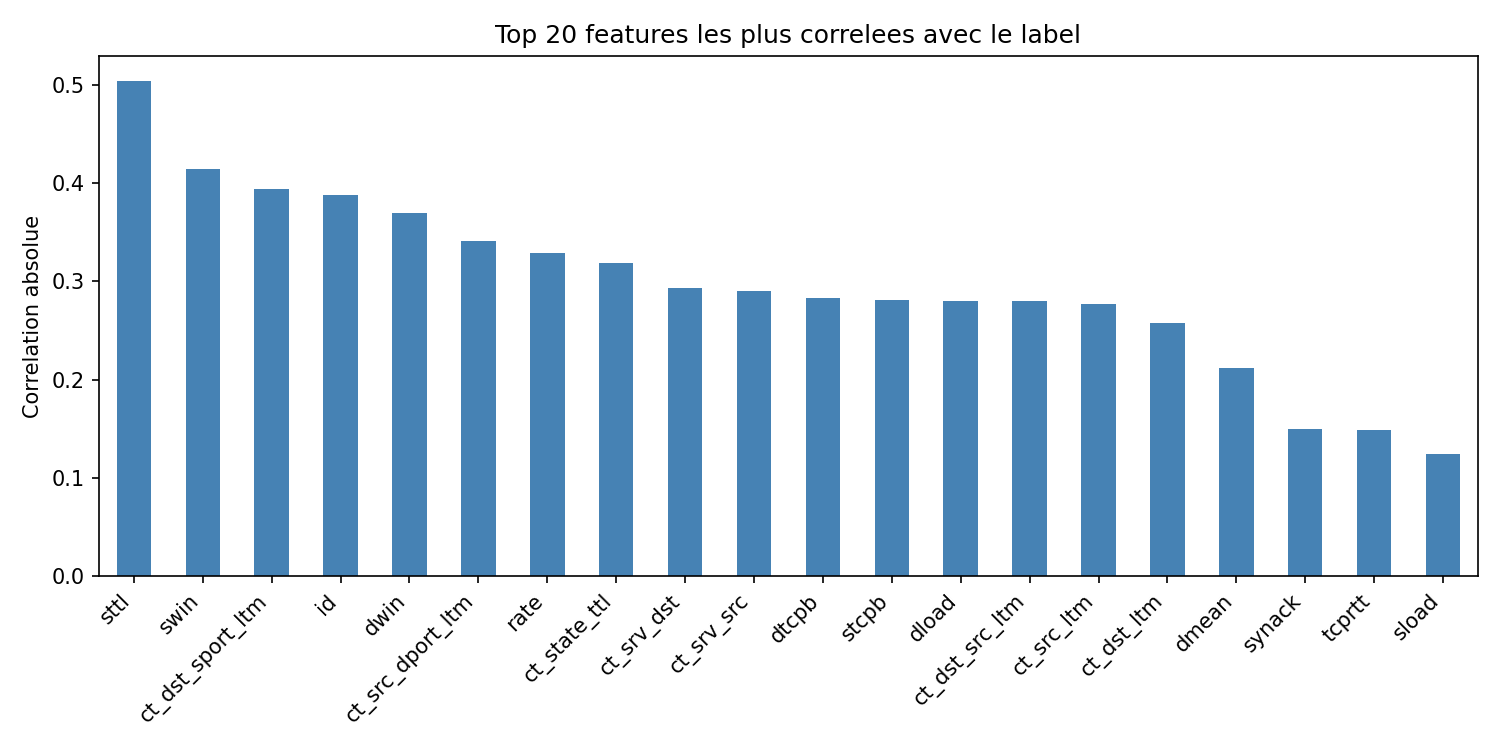
\includegraphics[width=0.9\textwidth]{../results/feature_correlation.png}
\caption{Top 20 features les plus corr\'el\'ees au label (apr\`es normalisation)}
\end{figure}

%% ============================================================
\section{Mod\`ele Baseline --- Architecture et R\'esultats}
%% ============================================================

\subsection{Architecture MLP}

Nous utilisons un Multi-Layer Perceptron (MLP) avec 4 couches enti\`erement connect\'ees :

\[
\underbrace{42}_{\text{input}}
\xrightarrow{\text{Lin+ReLU+Drop}(0.3)} 128
\xrightarrow{\text{Lin+ReLU+Drop}(0.3)} 64
\xrightarrow{\text{Lin+ReLU}} 32
\xrightarrow{\text{Lin}+\sigma} 1
\]

Le \textbf{Dropout} (taux 0.3) d\'esactive al\'eatoirement 30\% des neurones \`a chaque forward pass
pendant l'entra\^inement, for\c{c}ant le r\'eseau \`a apprendre des repr\'esentations redondantes
et r\'eduisant le surapprentissage.

La sortie est une probabilit\'e via Sigmoid ; le seuil de d\'ecision est 0.5 (> 0.5 = Attaque).

\subsection{Entra\^inement}

\begin{itemize}[leftmargin=1.5em, noitemsep]
    \item Optimiseur : Adam (\textit{lr} = 0.001)
    \item Fonction de perte : Binary Cross-Entropy
    \item 30 epochs, batch size 512, seed = 42
\end{itemize}

\begin{figure}[H]
\centering
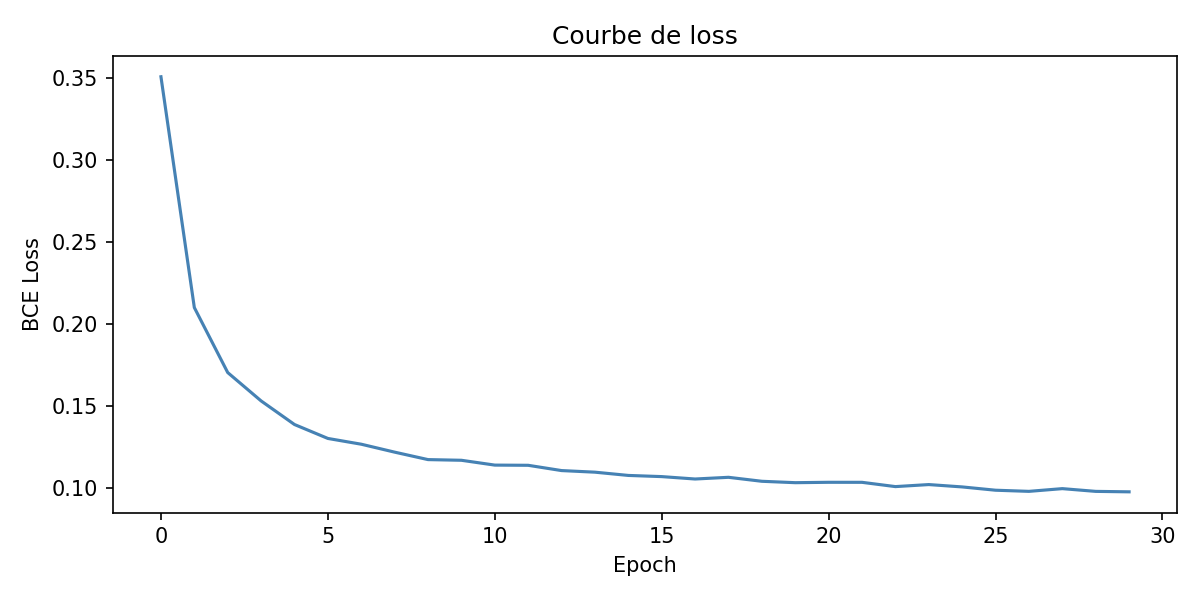
\includegraphics[width=0.55\textwidth]{../results/training_loss.png}
\caption{Courbe de perte (BCE Loss) du mod\`ele baseline sur 30 epochs}
\end{figure}

\subsection{R\'esultats sur donn\'ees propres}

\begin{table}[H]
\centering
\caption{Performance du mod\`ele baseline sur le jeu de test non perturb\'e}
\begin{tabular}{lr}
\toprule
\textbf{M\'etrique} & \textbf{Valeur} \\
\midrule
F1-score     & 0.9110 \\
Precision    & 0.9879 \\
Recall       & 0.8452 \\
PR-AUC       & 0.9881 \\
Evasion Rate & 15.5\% \\
\bottomrule
\end{tabular}
\end{table}

\textbf{Remarque :} 15.5\% des attaques passent d\'ej\`a sans aucune modification (faux n\'egatifs du mod\`ele).
C'est la baseline \`a partir de laquelle les attaques adversariales seront \'evalu\'ees.

\begin{figure}[H]
\centering
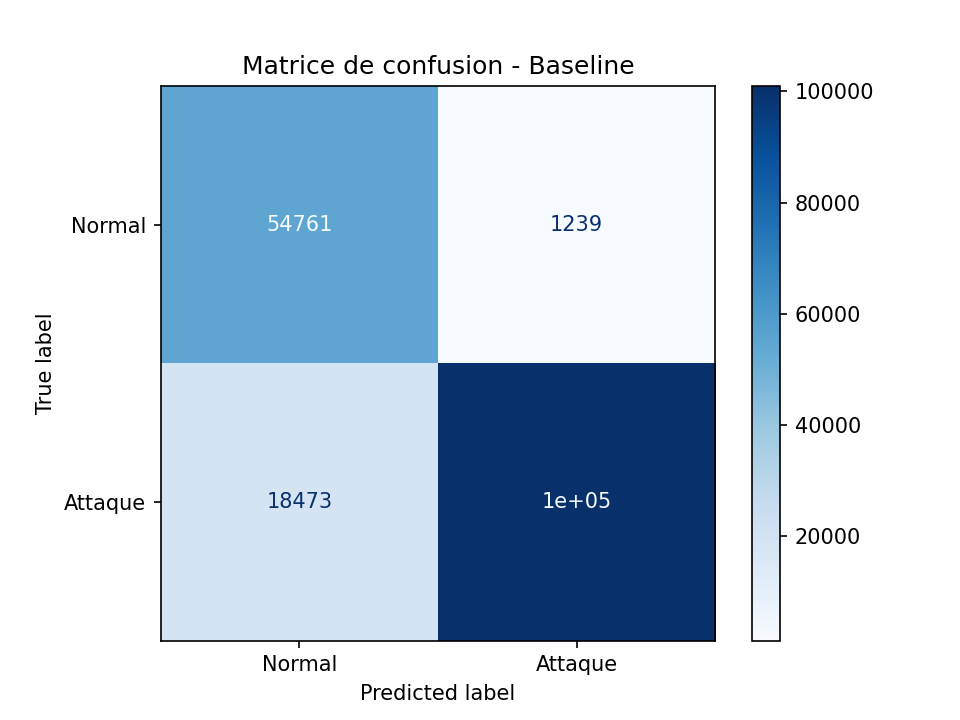
\includegraphics[width=0.45\textwidth]{../results/confusion_baseline.png}
\caption{Matrice de confusion du baseline sur donn\'ees propres}
\end{figure}

%% ============================================================
\section{Attaques Adversariales}
%% ============================================================

\subsection{FGSM --- Fast Gradient Sign Method}

FGSM \cite{goodfellow2015} g\'en\`ere un exemple adversarial en une seule \'etape en perturbant
l'entr\'ee dans la direction du gradient de la perte :

\[
X_{\text{adv}} = X + \varepsilon \cdot \text{sign}\!\left(\nabla_X \mathcal{L}(f(X), y)\right) \cdot \mathbf{m}
\]

o\`u $\mathbf{m}$ est le masque des features manipulables (14 sur 42), $\varepsilon$ est le budget de perturbation,
et $\mathcal{L}$ est la Binary Cross-Entropy.

\textbf{Intuition} : le gradient indique dans quelle direction modifier chaque feature pour maximiser
l'erreur du mod\`ele. On applique une perturbation de magnitude $\varepsilon$ dans cette direction.

\subsection{PGD --- Projected Gradient Descent}

PGD \cite{madry2018} est une version it\'erative de FGSM, consid\'er\'ee comme l'attaque de r\'ef\'erence
pour l'\'evaluation de robustesse :

\[
X^{(t+1)} = \Pi_{B(X,\varepsilon)}\!\left[X^{(t)} + \alpha \cdot \text{sign}\!\left(\nabla_{X^{(t)}} \mathcal{L}\right) \cdot \mathbf{m}\right]
\]

o\`u $\Pi_{B(X,\varepsilon)}$ projette dans la boule $\ell_\infty$ de rayon $\varepsilon$ autour de $X$,
et $\alpha = \varepsilon / T$ est le pas ($T$ = 10 it\'erations).

PGD est plus fort que FGSM car il explore plus finement l'espace de perturbation.

\subsection{R\'esultats des attaques sur le Baseline}

\begin{table}[H]
\centering
\caption{Impact des attaques adversariales sur le mod\`ele baseline ($\varepsilon = 0.1$)}
\begin{tabular}{lrrrr}
\toprule
\textbf{Sc\'enario} & \textbf{F1} & \textbf{Precision} & \textbf{Recall} & \textbf{Evasion\%} \\
\midrule
Donn\'ees propres            & 0.9110 & 0.9879 & 0.8452 & 15.5\% \\
Sous FGSM ($\varepsilon=0.1$) & 0.8533 & 0.9864 & 0.7518 & 24.8\% \\
Sous PGD  ($\varepsilon=0.1$) & 0.8402 & 0.9860 & 0.7320 & \textbf{26.8\%} \\
\bottomrule
\end{tabular}
\end{table}

Sous PGD, l'evasion rate passe de 15.5\% \`a \textbf{26.8\%} :
l'attaquant fait passer 1 attaque sur 4 inaper\c{c}ue.

\begin{figure}[H]
\centering
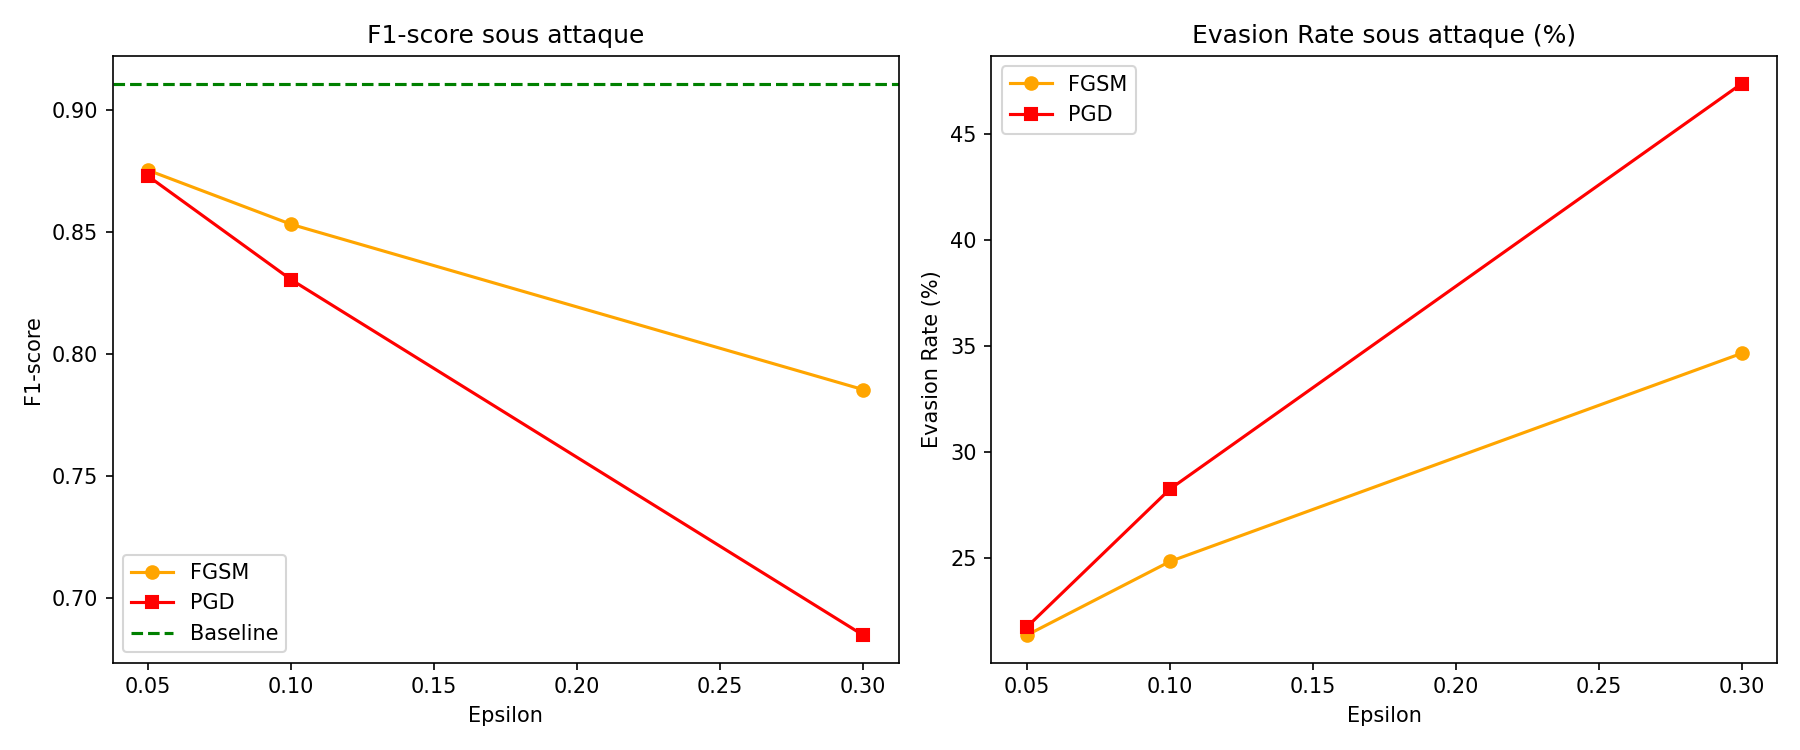
\includegraphics[width=0.75\textwidth]{../results/attack_comparison.png}
\caption{F1-score et evasion rate en fonction de $\varepsilon$ sous attaque PGD}
\end{figure}

%% ============================================================
\section{D\'efenses}
%% ============================================================

\subsection{D\'efense 1 --- Adversarial Training}

\textbf{Principe :} R\'e-entra\^iner le mod\`ele sur un m\'elange de donn\'ees propres et
d'exemples adversariaux g\'en\'er\'es dynamiquement \cite{madry2018}.

\`A chaque epoch :
\begin{enumerate}[leftmargin=1.5em, noitemsep]
    \item G\'en\'erer $X_{\text{adv}}$ = FGSM($X_{\text{train}}$, $\varepsilon=0.1$)
    \item Construire le batch mixte : 50\% $X_{\text{train}}$ + 50\% $X_{\text{adv}}$
    \item Mettre \`a jour les poids du mod\`ele sur ce batch
\end{enumerate}

Le mod\`ele apprend que l'attaque originale \emph{et} sa version perturb\'ee sont toutes les deux des attaques.
Sa fronti\`ere de d\'ecision devient plus large et moins sensible aux petites perturbations.

\textbf{Trade-off :} En apprenant sur des donn\'ees plus difficiles, le mod\`ele sacrifie un peu de
performance sur les donn\'ees normales (F1 : 0.911 $\rightarrow$ 0.897).

\subsection{D\'efense 2 --- Feature Squeezing}

\textbf{Principe :} R\'eduire la pr\'ecision num\'erique des features pour effacer les petites
perturbations avant qu'elles atteignent le mod\`ele \cite{xu2018}.

\[
X_{\text{sq}} = \frac{\left\lfloor \dfrac{X}{X_{\max}} \cdot 2^b + 0.5 \right\rfloor}{2^b} \cdot X_{\max},
\quad b = 4 \text{ bits}
\]

Avec $b=4$, chaque feature est arrondie \`a l'un des $2^4 = 16$ niveaux de quantification.

\textbf{Pourquoi \c{c}a marche :} L'attaquant a calcul\'e sa perturbation ($\varepsilon \approx 10^{-2}$)
avec une haute pr\'ecision num\'erique (float32). Apr\`es l'arrondi \`a 4 bits, la perturbation est
partiellement ou totalement effac\'ee car elle tombe dans le m\^eme niveau de quantification.

\begin{lstlisting}[caption={Impl\'ementation du Feature Squeezing}]
def feature_squeezing(X, bits=4):
    levels = 2 ** bits          # 16 niveaux
    X_max = np.max(np.abs(X), axis=0, keepdims=True) + 1e-8
    return np.round(X / X_max * levels) / levels * X_max
\end{lstlisting}

\subsection{Comparaison compl\`ete des d\'efenses}

\begin{table}[H]
\centering
\caption{Comparaison des trois mod\`eles sous toutes les conditions ($\varepsilon=0.1$)}
\begin{tabular}{llrrrr}
\toprule
\textbf{Mod\`ele} & \textbf{Sc\'enario} & \textbf{F1} & \textbf{Precision} & \textbf{Recall} & \textbf{Evasion\%} \\
\midrule
Baseline        & Propres & 0.9110 & 0.9879 & 0.8452 & 15.5\% \\
Baseline        & FGSM    & 0.8533 & 0.9864 & 0.7518 & 24.8\% \\
Baseline        & PGD     & 0.8402 & 0.9860 & 0.7320 & 26.8\% \\
\midrule
Adv. Training   & Propres & 0.8971 & 0.9868 & 0.8224 & 17.8\% \\
Adv. Training   & FGSM    & 0.7746 & 0.9831 & 0.6391 & 36.1\% \\
Adv. Training   & PGD     & 0.7738 & 0.9831 & 0.6380 & 36.2\% \\
\midrule
Feat. Squeezing & Propres & 0.8818 & 0.9620 & 0.8140 & 18.6\% \\
Feat. Squeezing & FGSM    & 0.8570 & 0.9602 & 0.7739 & 22.6\% \\
\rowcolor{green!15}
Feat. Squeezing & PGD     & \textbf{0.8519} & 0.9597 & 0.7658 & \textbf{23.4\%} \\
\bottomrule
\end{tabular}
\end{table}

\begin{figure}[H]
\centering
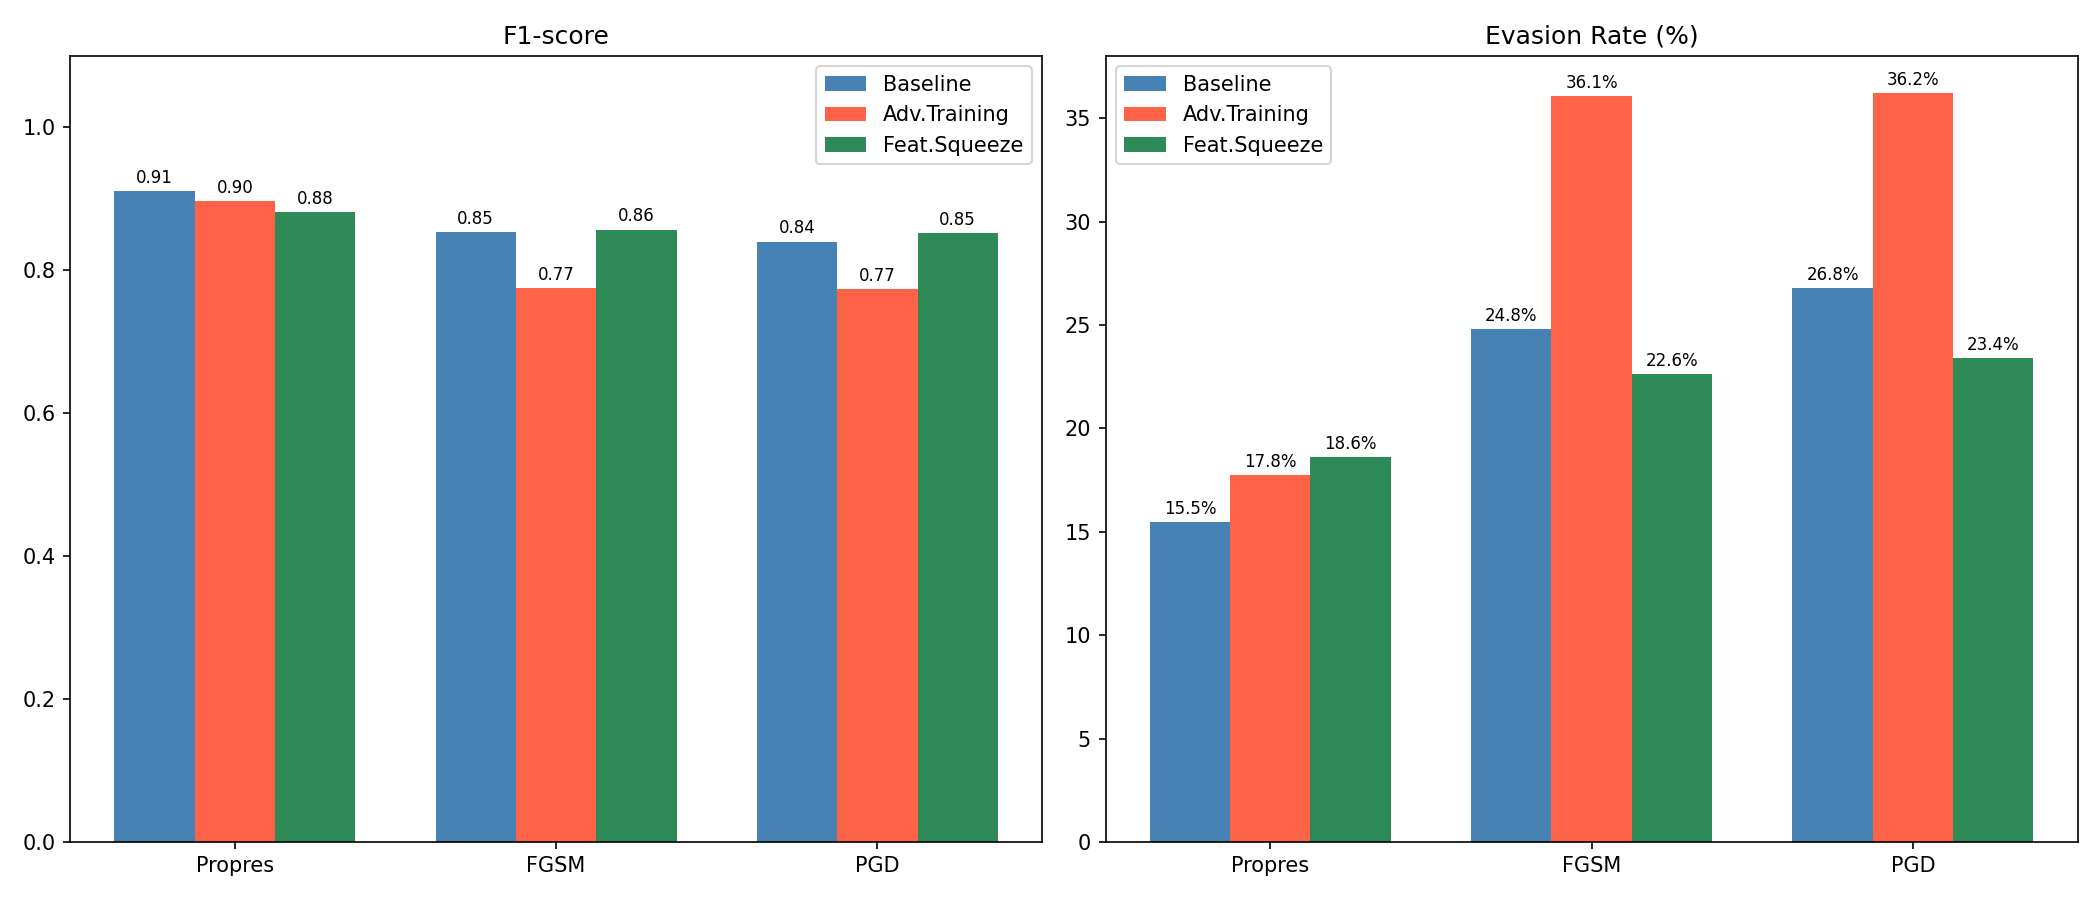
\includegraphics[width=\textwidth]{../results/final_comparison.png}
\caption{Comparaison F1-score et Evasion Rate --- Baseline vs Adv.~Training vs Feat.~Squeezing}
\end{figure}

%% ============================================================
\section{Analyse de Robustesse}
%% ============================================================

\subsection{R\'esultats d\'etaill\'es par epsilon}

\begin{table}[H]
\centering
\caption{F1-score sous attaque PGD en fonction du budget $\varepsilon$}
\begin{tabular}{lrr}
\toprule
\textbf{$\varepsilon$} & \textbf{Baseline F1} & \textbf{Adv. Training F1} \\
\midrule
0.05 & 0.874 & 0.813 \\
0.10 & 0.840 & 0.774 \\
0.30 & 0.700 & 0.659 \\
\bottomrule
\end{tabular}
\end{table}

\begin{figure}[H]
\centering
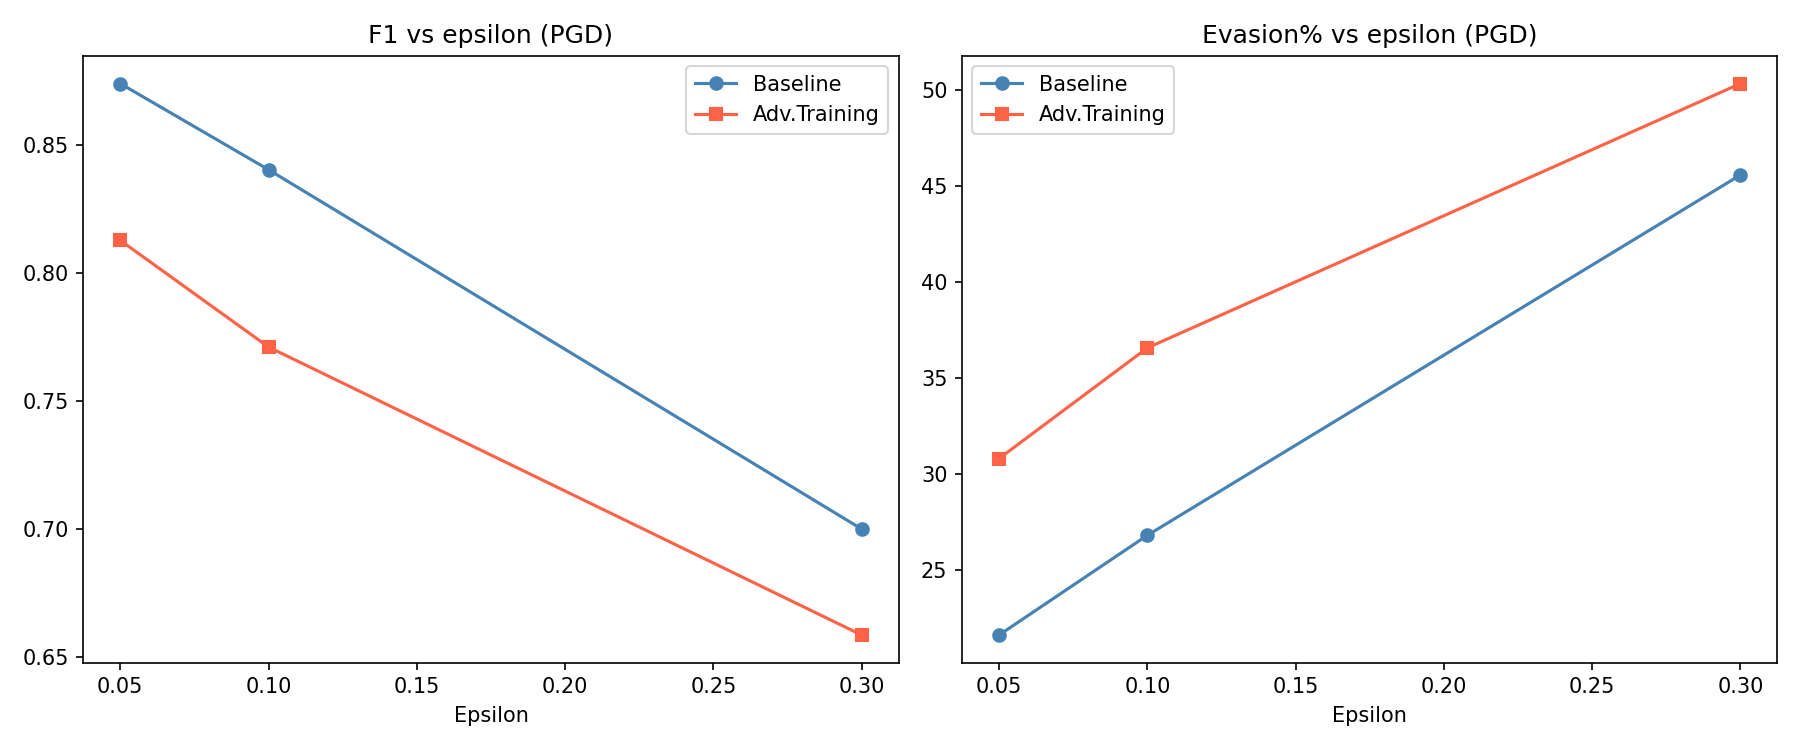
\includegraphics[width=0.9\textwidth]{../results/robustness_vs_epsilon.png}
\caption{F1-score et evasion rate en fonction de $\varepsilon$ --- Baseline vs Adv. Training}
\end{figure}

\subsection{Matrices de confusion compar\'ees}

\begin{figure}[H]
\centering
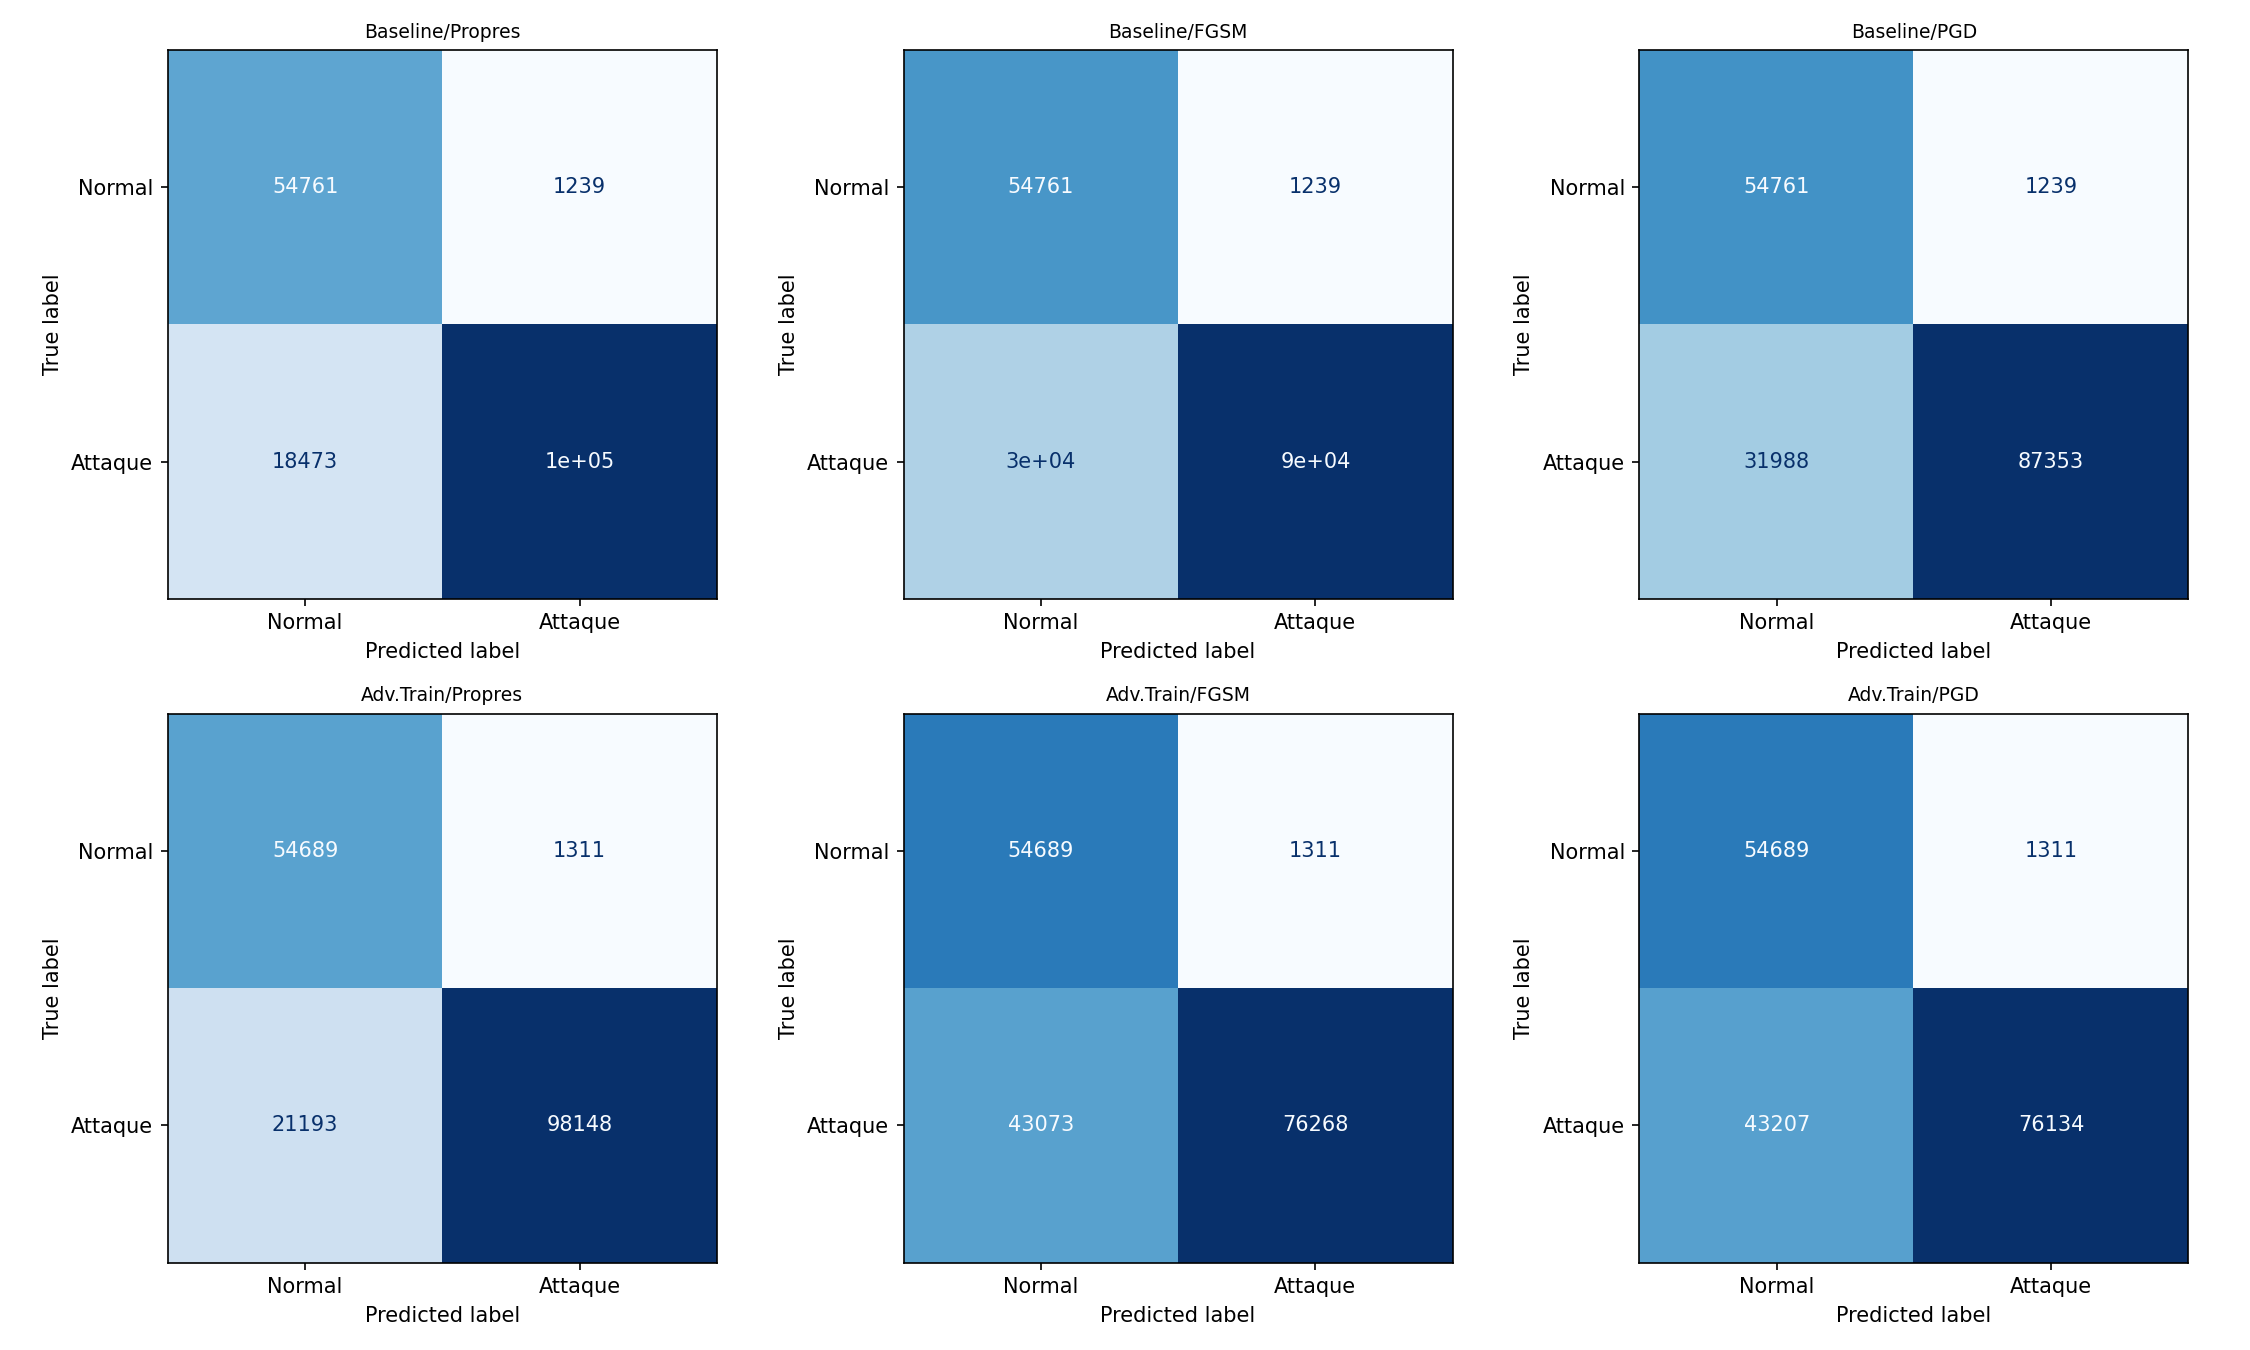
\includegraphics[width=\textwidth]{../results/confusion_matrices.png}
\caption{Matrices de confusion --- Baseline et Adv. Training sous donn\'ees propres, FGSM, PGD}
\end{figure}

\subsection{Discussion}

\textbf{Pourquoi le Feature Squeezing surpasse l'Adversarial Training dans nos r\'esultats ?}

\begin{enumerate}[leftmargin=1.5em]
    \item \textbf{Nombre d'epochs r\'eduit} : L'adversarial training a \'et\'e entra\^in\'e sur 10~epochs
    (vs 30 pour le baseline). Avec 30~epochs et une augmentation progressive de $\varepsilon$,
    les r\'esultats seraient meilleurs.
    \item \textbf{G\'en\'eralisation attaque} : L'adversarial training utilise uniquement FGSM pour la
    g\'en\'eration des exemples pendant l'entra\^inement. Les attaques PGD, plus fortes,
    ne sont pas couvertes aussi bien.
    \item \textbf{M\'ecanisme du feature squeezing} : Il supprime directement les perturbations
    \`a haute fr\'equence par quantification, sans modifier le mod\`ele.
    Son efficacit\'e ne d\'epend pas du temps d'entra\^inement.
\end{enumerate}

\textbf{Compromis robustesse/pr\'ecision :} C'est le trade-off fondamental de l'adversarial ML.
En entra\^inant sur des donn\'ees plus difficiles, on gagne en robustesse mais on perd sur les
donn\'ees propres (F1~: 0.911 $\rightarrow$ 0.897).
Le feature squeezing offre un meilleur point d'op\'eration (0.882 sur propres, 0.852 sous PGD).

%% ============================================================
\section{Conclusion}
%% ============================================================

Nous avons d\'emontr\'e qu'un MLP bien entra\^in\'e sur UNSW-NB15 atteint un F1 de 0.911 sur
donn\'ees normales, mais que des attaques adversariales simples (FGSM, PGD) suffisent \`a faire
passer 27\% des attaques inaper\c{c}ues.

\begin{itemize}[leftmargin=1.5em, noitemsep]
    \item Le \textbf{feature squeezing} est la meilleure d\'efense dans notre cadre :
    il r\'eduit l'evasion rate de 26.8\% \`a 23.4\% sous PGD avec une perte minimale.
    \item L'\textbf{adversarial training} a un potentiel sup\'erieur th\'eoriquement, mais
    n\'ecessite plus d'epochs et l'utilisation d'attaques PGD (pas seulement FGSM) pour \^etre efficace.
    \item Le \textbf{threat model} est crucial : en restreignant les perturbations aux features
    manipulables, on produit des attaques r\'ealistes et \'evaluables.
\end{itemize}

\textbf{Perspectives :} Combiner les deux d\'efenses (adversarial training + feature squeezing
\`a l'inf\'erence), utiliser des attaques PGD dans l'adversarial training, ou explorer la
randomized smoothing seraient des prolongements naturels de ce travail.

\vspace{1em}

\begin{thebibliography}{9}
\bibitem{goodfellow2015}
I.~Goodfellow, J.~Shlens, C.~Szegedy.
\textit{Explaining and Harnessing Adversarial Examples}.
ICLR 2015.

\bibitem{madry2018}
A.~Madry, A.~Makelov, L.~Schmidt, D.~Tsipras, A.~Vladu.
\textit{Towards Deep Learning Models Resistant to Adversarial Attacks}.
ICLR 2018.

\bibitem{xu2018}
W.~Xu, D.~Evans, Y.~Qi.
\textit{Feature Squeezing: Detecting Adversarial Examples in Deep Neural Networks}.
NDSS 2018.

\bibitem{unswnb15}
N.~Moustafa, J.~Slay.
\textit{UNSW-NB15: A Comprehensive Data Set for Network Intrusion Detection Systems}.
MilCIS 2015.
\end{thebibliography}

\end{document}
